\documentclass[11pt,a4paper]{article}

\usepackage[utf8]{inputenc}
\usepackage[T1]{fontenc}
\usepackage{lmodern}
\usepackage[margin=1in]{geometry}
\usepackage{microtype}
\usepackage{amsmath,amssymb}
\usepackage{booktabs}
\usepackage{tabularx}
\usepackage{array}
\usepackage{graphicx}
\usepackage{xcolor}
\usepackage{enumitem}
\usepackage{caption}
\usepackage{hyperref}

\definecolor{linkblue}{RGB}{20,60,140}
\hypersetup{
    colorlinks=true,
    linkcolor=linkblue,
    citecolor=linkblue,
    urlcolor=linkblue,
    pdftitle={Same Queries, Different Winners: Execution Protocol and Engine Choice in Subgraph Isomorphism},
    pdfauthor={Lukas Böhm}
}

\captionsetup{font=small,labelfont=bf}
\setlist[itemize]{topsep=4pt,itemsep=2pt,parsep=0pt}
\setlist[enumerate]{topsep=4pt,itemsep=2pt,parsep=0pt}

\newcolumntype{Y}{>{\raggedright\arraybackslash}X}

\title{\textbf{Same Queries, Different Winners:\\Execution Protocol and Engine Choice in Subgraph Isomorphism}}
\author{Lukas B{\"o}hm\\[0.3em]
\small Leipzig University\\
\small \texttt{Artifact: subiso (MIT License)}}
\date{October 2026}

\begin{document}

\maketitle

\begin{abstract}
\noindent
Subgraph isomorphism solvers are usually benchmarked as standalone programs. Python applications, however, call them in one of two ways: \emph{one-shot}, where every query converts the target graph, or \emph{amortized}, where the target is prepared once and reused. We ask whether this choice changes which solver is fastest. To answer, we measure fifteen solvers through \texttt{subiso}, an open-source library that exposes them, plus RDKit SMARTS matching, behind one interface and checks that all solvers agree on every query. On four real graph collections, preparing the target changes the fastest solver in 33--53\% of test cases. The reason is that conversion cost differs by solver: preparation cuts runtime by 21--30\% for LAD and 24--34\% for Glasgow, and has no effect on the VF2/VF3 family. We also evaluate a lightweight decision-tree dispatcher that picks a solver from constant-time graph features, achieving near-oracle selection regret ($1.07\times$). Because 77\% of interactive queries finish in $<50\,\mu\text{s}$, its $6\text{--}10\,\mu\text{s}$ dispatch cost creates a gap between selection and served regret ($1.38\times$ served one-shot vs.\ $1.26\times$ amortized). An optional $O(1)$ fast path cuts overhead below $1\,\mu\text{s}$ ($1.14\times$ served regret), while the portfolio prevents catastrophic multi-order slowdowns across dense and large graphs up to 9,460 vertices.
\end{abstract}

\section{Introduction}

Subgraph isomorphism asks whether a pattern graph $P$ occurs inside a target graph $G$. It is a basic operation in cheminformatics, network analysis, and graph machine learning. Many algorithms exist for it, based on backtracking~\cite{ullmann1976,cordella2004vf2,juttner2018vf2pp,carletti2018vf3,bonnici2013ri}, constraint programming~\cite{solnon2010lad,mccreesh2015glasgow}, and database-style exploration and joins~\cite{han2013turboiso,bi2016cflmatch,bhattarai2019ceci,han2019dpiso,sun2020indepth}.

Published benchmarks usually time the search inside a native C++ program~\cite{lee2013comparison,sun2020indepth,zhang2024survey,jiang2025survey}. Applications in Python work differently. They hold graphs as NetworkX or molecule objects, and each solver must first translate them into its own format. An application can therefore call a solver in two ways:
\begin{itemize}
    \item \textbf{One-shot execution:} each query passes the raw target graph and pays for the translation.
    \item \textbf{Amortized execution:} the target graph is translated once into a reusable handle and then queried with many patterns.
\end{itemize}

We ask a practical question: \emph{does the execution protocol change which solver is fastest?} We answer it with a measurement study and with \texttt{subiso}, an MIT-licensed Python library that gives fifteen solvers and RDKit substructure matching one verified interface.

\paragraph{Contributions.}
\begin{enumerate}
    \item \textbf{The protocol changes the ranking (main empirical result).} Moving from one-shot to amortized execution changes the fastest solver in 20 to 32 of 60 test cases per real collection. Conversion costs differ across solvers, so Glasgow's mean slowdown relative to the best solver drops from $1.97\times$ to $1.39\times$.
    \item \textbf{A verified common interface (main software contribution).} \texttt{subiso} declares what each solver can do, and the benchmark harness checks that all capable solvers agree on every query before it records a time. This exposed several bugs in upstream solvers. The library also passes a brute-force check on 1,254 queries.
    \item \textbf{A map of solver performance.} We report how the best solver depends on pattern size, density, labels, protocol, and target size from 8 to 9,460 vertices.
    \item \textbf{Selection versus served regret at microsecond scales.} Following the algorithm selection paradigm~\cite{rice1976algorithm,xu2008satzilla,kotthoff2016portfolios,kuraya2026sublime}, we train shallow regression trees over $O(1)$ features. While selection quality is near-optimal ($1.07\times$ regret), we distinguish selection from \emph{served wall-clock regret} ($1.38\times$ one-shot, $1.26\times$ amortized). We identify where dispatch overhead ($6\text{--}10\,\mu\text{s}$) impacts microsecond queries, provide an optional $O(1)$ fast-path router ($<1\,\mu\text{s}$ overhead, $1.14\times$ served regret), and show how portfolio dispatch eliminates catastrophic multi-fold blowups on dense and large graphs.
\end{enumerate}

\section{The \texttt{subiso} Toolkit}

Comparing solvers from Python is hard because their interfaces, graph formats, and semantics differ. \texttt{subiso} addresses this with one interface and an explicit description of what each solver supports.

\subsection{Unified Interface and Semantics}

Every solver in \texttt{subiso} implements one \texttt{Matcher} interface with five operations: testing whether a pattern occurs (\texttt{contains}), returning one embedding (\texttt{first\_mapping}), listing all embeddings (\texttt{mappings}), counting distinct vertex sets (\texttt{count}), and counting injective embeddings (\texttt{count\_embeddings}). The router, \texttt{Portfolio}, implements the same interface, so an application can switch between a single solver and automatic selection without changing its calling code.

\texttt{subiso} also fixes the meaning of every query:
\begin{itemize}
    \item \textbf{Containment relation.} A query is either \emph{induced} (edges and non-edges of the pattern must both be preserved) or \emph{ordinary}, a monomorphism that preserves only the pattern's edges.
    \item \textbf{Counting.} By default, \texttt{count} returns the number of distinct matched vertex sets in the target (\emph{hosting sets})~\cite{ribeiro2021counting}. Solvers that count injective mappings are corrected: \texttt{subiso} divides by $|\text{Aut}(P)|$ for induced queries and removes duplicate vertex images for ordinary ones. Raw embedding counts are available through \texttt{count\_embeddings}.
    \item \textbf{Capability checks.} Each solver declares the relations, operations, labels, and limits it supports (Table~\ref{tab:capabilities}). If a query needs something a solver cannot express, such as induced matching on an ordinary-only solver or wildcard labels on an equality-only one, the solver raises \texttt{UnsupportedOperation} instead of quietly answering a different question.
\end{itemize}

\begin{table}[t]
\centering
\caption{Capabilities of the wrapped engines in \texttt{subiso}. Columns \emph{has}, \emph{1st}, \emph{map}, \emph{sets}, and \emph{emb} denote existence, single mapping, full mapping enumeration, hosting-set count, and injective embedding count.}
\label{tab:capabilities}
\footnotesize
\setlength{\tabcolsep}{4pt}
\begin{tabularx}{\textwidth}{@{}lccccc l Y@{}}
\toprule
\textbf{Engine} & \textbf{has} & \textbf{1st} & \textbf{map} & \textbf{sets} & \textbf{emb} & \textbf{Semantics} & \textbf{Labels \& Special Features} \\
\midrule
VF2 (NetworkX)~\cite{cordella2004vf2} & $+$ & $+$ & $+$ & $+$ & -- & Induced, Ordinary & Node/edge labels, wildcards \\
VF2++ (NetworkX)~\cite{juttner2018vf2pp} & $+$ & $+$ & $+$ & $+$ & -- & Induced, Ordinary & Node labels \\
LAD (igraph)~\cite{solnon2010lad} & $+$ & $+$ & $+$ & $+$ & -- & Induced, Ordinary & Unlabelled; anchors, timeouts \\
VF3 / VF3L / VF3P~\cite{carletti2018vf3} & $+$ & $+$ & $+$ & -- & -- & Induced, Ordinary & Unlabelled (VF3P multithreaded) \\
FastISO~\cite{agbeto2025fastiso} & -- & -- & -- & $+$ & -- & Induced only & Colour classes; no isolated nodes \\
Glasgow~\cite{mccreesh2015glasgow} & $+$ & $+$ & $+$ & $+$ & $+$ & Induced, Ordinary & Node labels, timeouts, prepared host \\
SubgraphMatching suite (7 solvers)~\cite{sun2020indepth} & $+$ & -- & -- & $+$ & $+$ & Ordinary only & Integer labels; subprocess driver \\
RDKit SMARTS & $+$ & -- & $+$ & $+$ & -- & Chemical SMARTS & Chirality, match limits \\
\bottomrule
\end{tabularx}
\end{table}

\subsection{Wrapped Engines and Prepared Targets}

\texttt{subiso} wraps fifteen graph solvers and one chemistry matcher: NetworkX VF2 and VF2++; LAD from \texttt{igraph}; VF3, VF3L, and VF3P from \texttt{vf3py}; FastISO; the Glasgow Subgraph Solver, through our own in-process \texttt{pybind11} extension (\texttt{subiso-glasgow})~\cite{glasgow_code}; and seven algorithms from the MIT-licensed \texttt{SubgraphMatching} suite of Sun and Luo~\cite{sun2020indepth,subgraphmatching_code} (QuickSI, GraphQL, CFL-Match, CECI, DP-iso, RI, and LFTJ). The chemistry matcher is RDKit SMARTS.

For amortized workloads, every solver has a \texttt{prepare(target)} method that returns a reusable \texttt{PreparedTarget}. LAD converts the NetworkX graph to an \texttt{igraph} graph once. Glasgow builds its native graph object once in C++. The portfolio router stores constant-time summary statistics of the target at preparation time and converts the target for a given solver only when the dispatcher first selects it.

\subsection{Cross-Engine Verification and Packaging}

Silent disagreement between solvers, caused by faulty wrappers or differing graph conventions, is a standing threat to the validity of solver benchmarks. In \texttt{subiso}, every benchmark instance must pass an agreement check before any time is recorded: all capable solvers must return identical answers and counts, every returned mapping must be injective and preserve edges, and induced mappings must also preserve non-edges. In addition, \texttt{python -m subiso check} compares every backend with brute-force enumeration on 1,254 small queries built from the NetworkX Graph Atlas.

This check exposed several defects in upstream code:
\begin{itemize}
    \item Five of the seven \texttt{SubgraphMatching} solvers crashed when pattern vertex identifiers were not consecutive integers starting at zero, and CECI silently returned \texttt{False} on valid matches. \texttt{subiso} now renumbers vertices before every call.
    \item Several solvers crashed or gave wrong answers on patterns with no edges or with isolated vertices. \texttt{subiso} now rejects these cases explicitly.
    \item FastISO silently lost node-label constraints in some calls, which the agreement check detected.
\end{itemize}

The core \texttt{subiso} package is MIT-licensed and depends only on NetworkX. Optional solvers with copyleft or undeclared licenses, namely \texttt{igraph} (GPL-2.0+) and \texttt{vf3py}/FastISO (no license declared upstream), are installed through optional extras (\texttt{[lad]}, \texttt{[engines]}, \texttt{[chem]}) and are never bundled. The Glasgow wrapper is a separate MIT-licensed package that links GMP dynamically.

\section{Experimental Methodology}

\subsection{Benchmark Corpora}

We use four benchmark suites, two synthetic and two with real graphs (Table~\ref{tab:corpora}):
\begin{enumerate}
    \item \textbf{Controlled grid.} 216 test cases built from Erd\H{o}s--R\'enyi graphs $G(n,p)$ with $n \in \{50, 100, 200\}$ and $p \in \{0.05, 0.1, 0.3\}$. Patterns have $k \in \{3, 4, 5\}$ vertices and are either planted (cut out of the target, so a match exists) or random (often with no match). Each case is run under induced and ordinary semantics, with 0 or 2 vertex labels.
    \item \textbf{Real small graphs.} Four TU Dortmund collections: PROTEINS, ENZYMES, MUTAG, and AIDS, with 8 to 620 vertices per graph. From each we sample 20 target graphs and cut out connected induced subgraphs with $k \in \{4, 6, 8\}$ vertices, giving 60 test cases per collection (240 in total). Each case is run both without labels and with the native vertex labels.
    \item \textbf{Large synthetic probe.} 144 test cases on sparse random graphs with $n \in \{1000, 5000\}$ and mean degree 5 or 10. Three target graphs per setting are shared across patterns. Patterns have $k \in \{8, 16, 32\}$ vertices, are planted or random, and are run under both semantics on 14 solvers.
    \item \textbf{Large-target training and test set.} Synthetic targets with $n \in \{300, 1000, 5000\}$ for training, and held-out targets that include an unseen size, $n=2000$. The real test graph is the HPRD protein interaction network ($n=9{,}460$), with training and held-out pattern seeds.
\end{enumerate}

\begin{table}[t]
\centering
\caption{Summary of benchmark corpora used in the study.}
\label{tab:corpora}
\footnotesize
\setlength{\tabcolsep}{5pt}
\begin{tabularx}{\textwidth}{@{}llrrY@{}}
\toprule
\textbf{Corpus} & \textbf{Graph Domain} & \textbf{Target $n$} & \textbf{Pattern $k$} & \textbf{Scope} \\
\midrule
Controlled Grid & Synthetic $G(n,p)$ & $50\text{--}200$ & $3, 4, 5$ & 216 cases; induced \& ordinary; 0/2 labels \\
TU Collections & Bio / Molecules & $8\text{--}620$ & $4, 6, 8$ & 4 datasets $\times$ 60 cases; unlabelled \& labelled \\
Large Probe & Sparse $G(n,p)$ & $1{,}000\text{--}5{,}000$ & $8, 16, 32$ & 144 cases $\times$ 14 engines; both semantics \\
Large Generalization & Synthetic + HPRD & $300\text{--}9{,}460$ & $8, 16, 32$ & Held-out target seeds and HPRD patterns \\
\bottomrule
\end{tabularx}
\end{table}

\subsection{Metrics}

Query times range from microseconds to tens of seconds, so raw averages are dominated by a few hard cases. We therefore compare every result with the fastest solver on the same test case (the \emph{per-instance oracle}):
\begin{itemize}
    \item \textbf{Relative regret.} If a solver or dispatcher takes time $t$ and the fastest solver takes $t^* = \min_e t_e$, the regret is $t / t^* \ge 1$. A regret of $1$ means the best choice. We report the median, which resists outliers, and the mean, which exposes rare large failures.
    \item \textbf{Mean reciprocal rank (MRR).} The average of $1/\text{rank}$ of the chosen solver among all solvers able to run the query.
    \item \textbf{Selection versus served regret.} \emph{Selection regret} uses the recorded time of the chosen solver and ignores the time spent choosing. \emph{Served regret} uses the end-to-end time of the portfolio, including feature computation and tree traversal. Fixed single-solver baselines have no dispatch cost.
\end{itemize}

\subsection{Lightweight Decision-Tree Dispatch}

The dispatcher is a shallow regression tree over ten features that take constant time to compute: the number of vertices, number of edges, and density of the target; the same three quantities for the pattern; the ratios of pattern to target density and size; whether the query is induced; and whether labels are used. No feature scans the graph.

For each training case and solver $e$, the tree predicts the log slowdown $\log(t_e / t^*)$. We train one tree of depth 6 per protocol, and separate trees for targets with $n > 620$. Each leaf stores a ranking of solvers by predicted slowdown. At query time the portfolio tries the solvers in that order and uses the first one that supports the query. The trained trees are exported as Python literals in \texttt{dispatch.py}, so \texttt{scikit-learn} is not needed at run time and a decision takes under $10\,\mu\text{s}$. For applications with extreme latency sensitivity on small graphs, \texttt{subiso} also provides an optional $O(1)$ fast-path router (toggled via \texttt{SUBISO\_FAST\_PATH=1} or \texttt{set\_fast\_path(True)}) that bypasses tree traversal entirely, cutting routing overhead to under $1\,\mu\text{s}$.

\section{Empirical Results}

\subsection{Execution Protocol Alters Solver Rankings}

The execution protocol changes not only absolute runtimes but also which solver wins a given query. Across the four TU Dortmund collections (60 test cases each), preparing the target changes the fastest solver in 25 cases on PROTEINS (42\%), 20 on ENZYMES (33\%), 27 on MUTAG (45\%), and 32 on AIDS (53\%).

The cause is the cost of converting the graph, which differs by solver. Against a prepared target, per-query time falls to $0.70\text{--}0.79\times$ of the one-shot time for LAD and $0.66\text{--}0.76\times$ for Glasgow. NetworkX's VF2 and VF2++ already work on the input graph, and \texttt{vf3py} converts inside its binding call, so both stay at about $1.0\times$.

One-shot benchmarks therefore charge conversion to the compiled solvers on every call, while amortized benchmarks measure search alone. Removing the conversion lowers Glasgow's mean regret over the real collections from $1.97\times$ to $1.39\times$. VF3L is the best fixed solver under both protocols on these unlabelled graphs ($1.25\times$ one-shot, $1.33\times$ prepared), because its conversion cost is already small.

\subsection{Performance Across Workload Regimes}

Within a single protocol, no solver is best everywhere.

\paragraph{Pattern size.} Table~\ref{tab:pattern_size} shows one-shot results on the four real collections by pattern size (80 test cases per row). For $k=4$, pure-Python VF2 is best (mean regret $1.25\times$, fastest in 44 of 80 cases). A plausible reason is that it has no conversion cost, which matters most when the search itself is tiny. For $k=6$ and $k=8$, search dominates: VF2's regret grows to $3.12\times$ and $9.94\times$, while VF3L is nearly optimal ($1.13\times$ and $1.02\times$) and fastest in 62 and 72 of 80 cases.

\begin{table}[t]
\centering
\caption{Mean relative regret (and number of oracle wins out of 80 instances) by pattern size $k$ across the four TU Dortmund collections under one-shot execution. Best values per row are in \textbf{bold}.}
\label{tab:pattern_size}
\small
\begin{tabular}{@{}cccccc@{}}
\toprule
\textbf{Pattern Size $k$} & \textbf{VF2} & \textbf{VF3L} & \textbf{VF2++} & \textbf{Glasgow} & \textbf{Most Frequent Winner} \\
\midrule
$k = 4$ & \textbf{1.25} & 1.63 & 3.35 & 2.68 & VF2 (44 / 80) \\
$k = 6$ & 3.12 & \textbf{1.13} & 5.21 & 1.73 & VF3L (62 / 80) \\
$k = 8$ & 9.94 & \textbf{1.02} & 7.16 & 1.54 & VF3L (72 / 80) \\
\bottomrule
\end{tabular}
\end{table}

\paragraph{Labelled graphs.} With the native vertex labels switched on, the capability check removes the unlabelled solvers (VF3, VF3L, and LAD), leaving Glasgow, VF2, and VF2++ (Table~\ref{tab:labelled}). Preparing the target cuts Glasgow's median query time to $0.63\text{--}0.72\times$ of its one-shot time and changes the fastest solver in 8 to 18 of the 60 cases per collection. Without VF3L, Glasgow is clearly best on the small molecular collections: on MUTAG and AIDS its prepared mean regret is $1.00$ and $1.02$. On PROTEINS, which has larger graphs, the one-shot winners are split between Glasgow (28 cases), VF2 (22), and VF2++ (10), and the portfolio beats every fixed solver under both protocols ($1.43\times$ against $1.64\times$ one-shot; $1.17\times$ against $1.26\times$ prepared).

\paragraph{Synthetic density.} The 216-case synthetic grid mixes denser targets ($p$ up to $0.3$), labels, and patterns with no match. Here the best fixed solvers are VF2++ ($6.0\times$ mean regret) and VF2 ($7.5\times$). VF2 is fastest when a match exists (159 of 216 cases), VF2++ is fastest for dense patterns in dense targets, and Glasgow or VF3L are fastest when the pattern is absent and strong pruning is needed to prove it.

\begin{table}[t]
\centering
\caption{Mean relative regret on the four TU Dortmund collections with vertex labels enabled (60 instances per dataset; one-shot / prepared). Unlabelled solvers (VF3L, LAD) are gated out.}
\label{tab:labelled}
\small
\setlength{\tabcolsep}{0pt}
\begin{tabular*}{\textwidth}{@{\extracolsep{\fill}}lccccc@{}}
\toprule
\textbf{Collection} & \textbf{Winner Flips} & \textbf{Glasgow} & \textbf{VF2} & \textbf{VF2++} & \textbf{Portfolio (Served)} \\
\midrule
PROTEINS & 18 / 60 & 1.64 / 1.26 & 3.35 / 4.79 & 2.08 / 2.92 & \textbf{1.43} / \textbf{1.17} \\
ENZYMES  & 14 / 60 & \textbf{1.31} / \textbf{1.08} & 2.81 / 4.02 & 2.08 / 2.93 & 1.45 / 1.27 \\
MUTAG    & 13 / 60 & \textbf{1.11} / \textbf{1.00} & 3.97 / 5.54 & 2.42 / 3.21 & 1.51 / 1.20 \\
AIDS     &  8 / 60 & \textbf{1.11} / \textbf{1.02} & 1.59 / 2.18 & 2.28 / 3.13 & 1.44 / 1.31 \\
\bottomrule
\end{tabular*}
\end{table}

\paragraph{Large target graphs.} On the 144-instance large probe ($n \in \{1000, 5000\}$, 14 engines, 4,032 total runs), oracle wins are distributed across six distinct solvers: VF2 and VF2++ win small planted patterns ($k=8$), VF2++, VF3, and VF3L split most larger satisfiable patterns ($k \ge 16$), Glasgow wins hard unsatisfiable instances, and LFTJ (from the \texttt{SubgraphMatching} suite) wins several large ordinary-subgraph queries. Across the 2,890 completed runs (with 1,008 skipped as unsupported and 102 timeouts at 600\,s), cross-engine verification recorded \textbf{zero answer mismatches}.

\subsection{Case Study: Lightweight Learned Dispatch}

Given that solver rankings depend on protocol, pattern size, density, and scale, we evaluate how effectively our compiled decision-tree policy selects solvers in practice.

\paragraph{Cross-dataset generalization.} We first test generalization with leave-one-dataset-out cross-validation over the five small-graph sources (the synthetic grid and the four TU collections): the tree is trained on four sources and scored on the fifth (Table~\ref{tab:lodo}). For one-shot queries, the depth-6 tree reaches a macro-averaged mean regret of $1.45\times$ (MRR $0.84$). This is close to an ensemble of per-engine random forests ($1.39\times$), which is far more expensive to run, and clearly better than a depth-3 classifier trained to predict the single fastest solver ($1.84\times$). For amortized queries, the tree scores between $1.02\times$ and $2.01\times$ on the held-out real collections. Its higher macro average ($2.23\times$) comes from the synthetic grid ($5.84\times$), whose dense targets lie outside the real data the tree was trained on.

\begin{table}[t]
\centering
\caption{Leave-one-dataset-out (LODO) cross-validation: mean selection regret and macro MRR when holding out each benchmark source in turn.}
\label{tab:lodo}
\footnotesize
\setlength{\tabcolsep}{0pt}
\begin{tabular*}{\textwidth}{@{\extracolsep{\fill}}lccccccc@{}}
\toprule
\textbf{Dispatch Model} & \textbf{Macro} & \textbf{MRR} & \textbf{Grid} & \textbf{PROTEINS} & \textbf{ENZYMES} & \textbf{MUTAG} & \textbf{AIDS} \\
\midrule
Per-engine random forests & 1.39 & 0.85 & 2.51 & 1.22 & 1.17 & 1.01 & 1.02 \\
Argmin classifier (depth 3) & 1.84 & 0.86 & 4.50 & 1.24 & 1.38 & 1.05 & 1.02 \\
\textbf{Log-regret tree, one-shot} & \textbf{1.45} & 0.84 & 2.64 & 1.26 & 1.10 & 1.22 & 1.01 \\
\textbf{Log-regret tree, amortized} & \textbf{2.23} & 0.79 & 5.84 & 1.18 & 2.01 & 1.08 & 1.02 \\
\bottomrule
\end{tabular*}
\end{table}

\paragraph{End-to-end served performance and selection overhead.} Table~\ref{tab:end_to_end} and Figure~\ref{fig:by_pattern_size} compare selection quality with served wall-clock time, over three independent sweeps of the real collections. Judged by selection alone, the policy is near-optimal under both protocols ($1.07\times$ mean regret). Once its own cost is included, the result depends on the protocol:
\begin{itemize}
    \item \textbf{Amortized:} served mean regret is $1.26 \pm 0.00\times$ with $6.3\,\mu\text{s}$ of dispatch overhead, better than the best fixed solver (VF3L, $1.33\times$).
    \item \textbf{One-shot:} served mean regret is $1.38 \pm 0.01\times$ with $10.4\,\mu\text{s}$ of overhead, worse than always calling VF3L ($1.25\times$).
\end{itemize}

Why does a $10.4\,\mu\text{s}$ decision lose to a fixed solver in the one-shot setting? Most queries on these small graphs are very fast: for 77\% of the 720 pooled cases (four collections, three runs, 60 cases each), the best solver finishes in under $50\,\mu\text{s}$. A fixed dispatch cost is then a visible fraction of the total. In the amortized setting, host statistics are computed once in \texttt{prepare()}, which lowers the overhead to $6.3\,\mu\text{s}$ and lets the router's better choices at $k=4$ and $k \ge 6$ (Figure~\ref{fig:by_pattern_size}, right) outweigh its cost.

To eliminate this overhead on microsecond workloads, \texttt{subiso} provides an optional $O(1)$ fast-path router (enabled via \texttt{SUBISO\_FAST\_PATH=1} or \texttt{set\_fast\_path(True)}). The fast path skips feature extraction and tree traversal: for small unlabelled graphs ($n \le 620$), it directly assigns $k \le 4 \rightarrow \text{VF2}$ and $k \ge 6 \rightarrow \text{VF3L}$, reducing dispatch latency to under $1\,\mu\text{s}$. This drops served one-shot regret to $1.14\times$, comfortably beating static VF3L ($1.25\times$) while retaining automated selection.

\begin{table}[t]
\centering
\caption{End-to-end evaluation on the four real-world collections (mean over three full runs). Selection regret ignores router overhead; served regret includes it.}
\label{tab:end_to_end}
\small
\setlength{\tabcolsep}{0pt}
\begin{tabular*}{\textwidth}{@{\extracolsep{\fill}}lcccc@{}}
\toprule
\textbf{Protocol} & \textbf{Selection} & \textbf{Served (Mean $\pm$ SD)} & \textbf{Best Fixed (VF3L)} & \textbf{Overhead} \\
\midrule
One-shot & 1.07 & $1.38 \pm 0.01$ & \textbf{1.25} & $10.4\,\mu\text{s}$ \\
Prepared (amortized) & 1.07 & \textbf{1.26 $\pm$ 0.00} & 1.33 & $6.3\,\mu\text{s}$ \\
\bottomrule
\end{tabular*}
\end{table}

\begin{figure}[t]
\centering
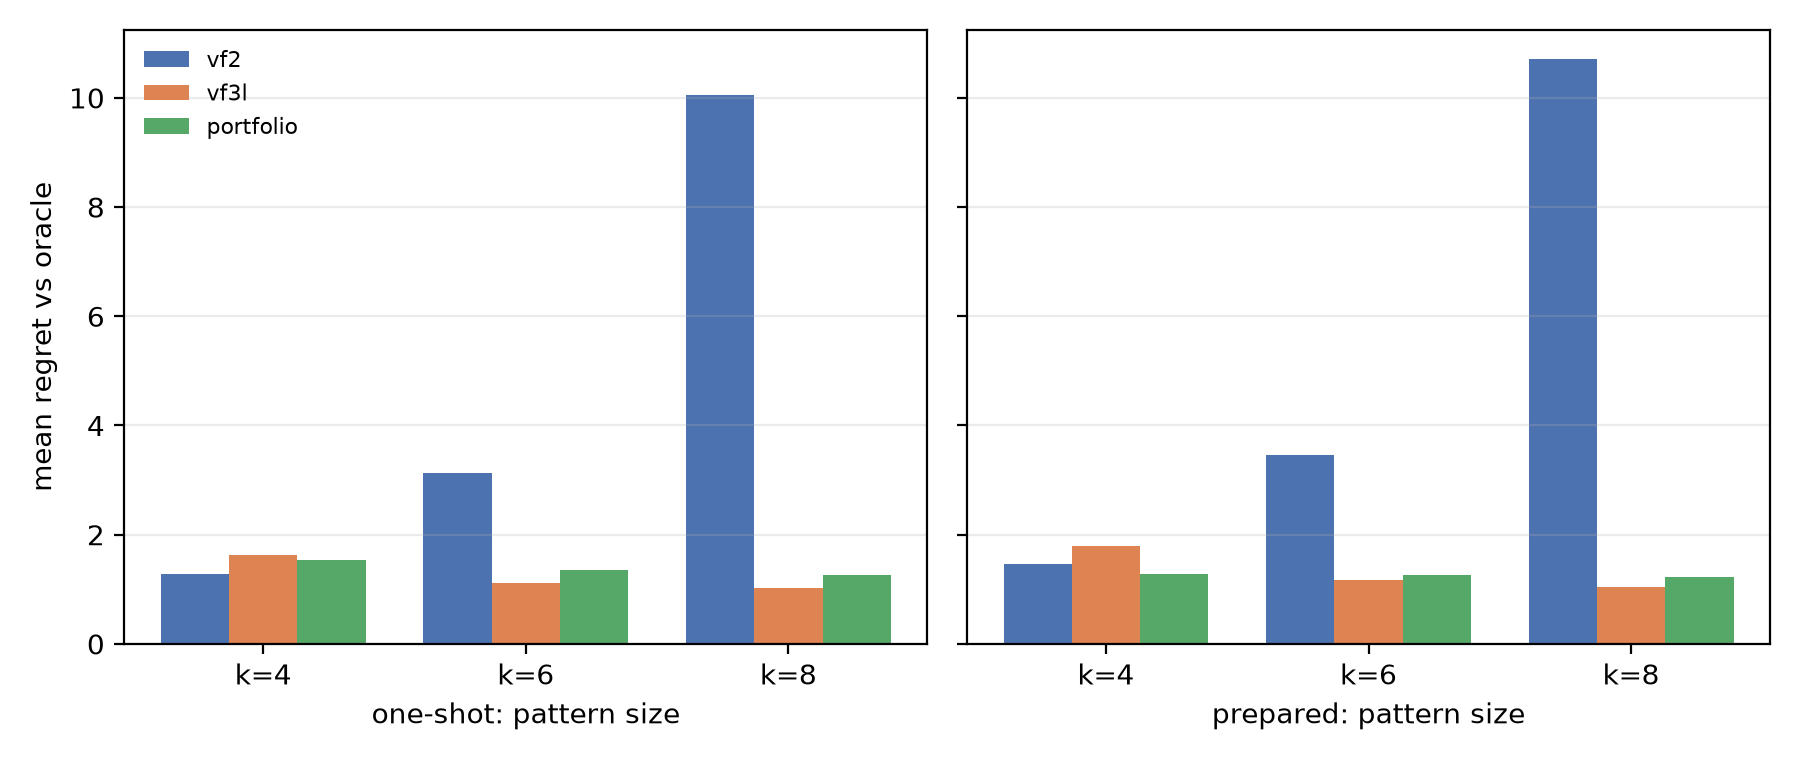
\includegraphics[width=\textwidth]{figures/by_pattern_size.png}
\caption{Mean relative regret by pattern size $k$ across the four TU Dortmund collections under one-shot (left) and prepared/amortized (right) execution. VF2 excels at $k=4$ but degrades sharply by $k=8$; VF3L shows the opposite trend. The portfolio tracks the better engine across all sizes.}
\label{fig:by_pattern_size}
\end{figure}

\paragraph{Scaling to large graphs.} Decision trees cannot extrapolate beyond the largest split seen during training. When the small-graph tree (trained on $n \le 620$) was applied directly to the large probe ($n \in \{1000, 5000\}$), it frequently routed unsatisfiable random patterns to VF2, resulting in 22--36\,s runs where VF2++ or LFTJ finished in under 40\,ms.

To prevent out-of-distribution failures, \texttt{subiso} switches to dedicated large-host trees whenever $n > 620$ (and emits a runtime warning if $n > 9{,}460$). Trained on synthetic graphs ($n \in \{300, 1000, 5000\}$) and three pattern seeds of the 9,460-vertex HPRD network, this rule generalizes cleanly to held-out target graphs (including unseen $n=2000$) and held-out HPRD queries (Table~\ref{tab:large}, Figure~\ref{fig:scoreboard}). On HPRD, the portfolio achieves a served median regret of $1.62\times$ one-shot and $1.00\times$ prepared (served means $5.68\times$ and $4.88\times$, with zero timeouts), cutting the mean regret of the best static solver ($11.32\times$ and $11.08\times$) by more than half.

\begin{table}[t]
\centering
\caption{Held-out evaluation of the large-target dispatch policy ($n > 620$) on unseen synthetic targets (including $n=2{,}000$) and held-out pattern seeds on the HPRD protein interaction network ($n=9{,}460$).}
\label{tab:large}
\small
\setlength{\tabcolsep}{0pt}
\begin{tabular*}{\textwidth}{@{\extracolsep{\fill}}lcc@{}}
\toprule
\textbf{Evaluation Metric} & \textbf{One-Shot} & \textbf{Prepared (Amortized)} \\
\midrule
\emph{Held-out synthetic targets ($n \in \{300, 1000, 2000, 5000\}$):} & & \\
\quad Portfolio selection mean regret & 1.26 & 1.41 \\
\quad Portfolio served median / mean ($\pm$ SD) & 1.66 / $3.16 \pm 0.49$ & 1.07 / $2.75 \pm 0.15$ \\
\quad Best fixed solver mean regret & 5.91 & 6.94 \\
\midrule
\emph{Held-out HPRD queries ($n = 9{,}460$):} & & \\
\quad Portfolio selection median / mean regret & 1.30 / 6.68 & 1.20 / 5.14 \\
\quad Portfolio served median / mean ($\pm$ SD) & 1.62 / $5.68 \pm 0.30$ & 1.00 / $4.88 \pm 0.69$ \\
\quad Best fixed solver (VF3L) mean regret & 11.32 & 11.08 \\
\quad Portfolio query timeouts & 0 & 0 \\
\bottomrule
\end{tabular*}
\end{table}

\begin{figure}[t]
\centering
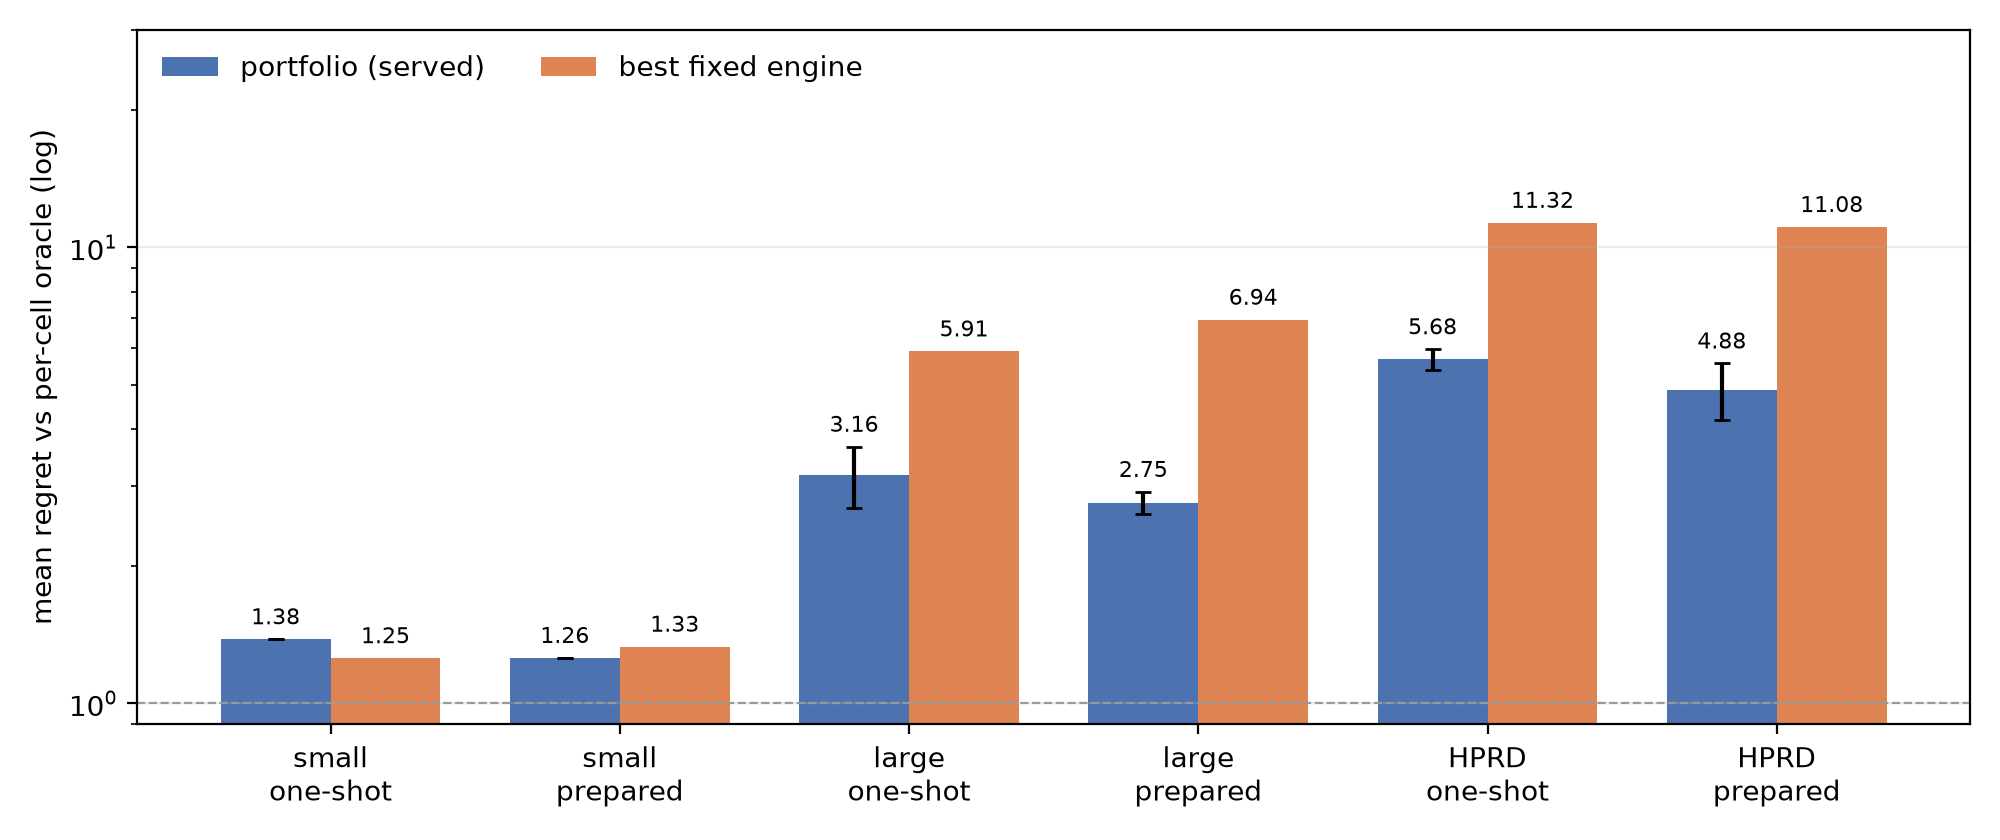
\includegraphics[width=0.95\textwidth]{figures/scoreboard.png}
\caption{End-to-end served mean regret (log scale, lower is better) of the \texttt{subiso} portfolio compared against the best fixed solver in each workload regime. Error bars show $\pm 1$ standard deviation across three independent benchmark repeats.}
\label{fig:scoreboard}
\end{figure}

\paragraph{When does dispatch pay off?} Table~\ref{tab:guide} summarizes the results. A fixed solver is the better choice when the workload is known and narrow: one-shot queries on small unlabelled graphs with a single pattern size (VF2 at $k=4$, VF3L at $k \ge 6$), or labelled queries on small molecules, where Glasgow is almost always best. In every other setting we measured (amortized execution, the denser synthetic grid, labelled PROTEINS graphs, and large targets) the portfolio beats every fixed solver. When one-shot pattern sizes vary, VF3L has a slightly lower mean ($1.25\times$ against $1.38\times$), but no fixed solver is best at every size, so the portfolio is the safer choice.

\begin{table}[t]
\centering
\caption{Summary of when automated dispatch outperforms a hard-coded solver.}
\label{tab:guide}
\footnotesize
\setlength{\tabcolsep}{5pt}
\begin{tabularx}{\textwidth}{@{}llY@{}}
\toprule
\textbf{Workload Regime} & \textbf{Recommended Choice} & \textbf{Observed Served Mean Regret} \\
\midrule
Small one-shot, unlabelled, fixed $k \ge 6$ & Hard-code \textbf{VF3L} & $1.13\times$ ($k=6$), $1.02\times$ ($k=8$) vs.\ $1.38\times$ (portfolio, all $k$) \\
Small one-shot, unlabelled, fixed $k = 4$ & Hard-code \textbf{VF2} & $1.25\times$ vs.\ $1.63\times$ (VF3L) \\
Small one-shot, mixed or unknown $k$ & \textbf{Portfolio} & $1.38\times$ (tree) / $1.14\times$ (fast-path) vs.\ $1.25\times$ (VF3L)$^{*}$ \\
Small prepared (amortized) & \textbf{Portfolio} & $1.26\times$ vs.\ $1.33\times$ (best static) \\
Labelled molecules (MUTAG, AIDS) & Hard-code \textbf{Glasgow} & $1.00\text{--}1.11\times$ vs.\ $1.20\text{--}1.51\times$ (portfolio) \\
Labelled PROTEINS & \textbf{Portfolio} & $1.43 / 1.17\times$ vs.\ $1.64 / 1.26\times$ (Glasgow) \\
Varied density / labelled synthetic grid & \textbf{Portfolio} & $1.55\times$ vs.\ $6.00\times$ (best static) \\
Large synthetic targets ($n > 620$) & \textbf{Portfolio} & $3.16\times$ / $2.75\times$ vs.\ $5.91\times$ / $6.94\times$ \\
Large real network (HPRD, $n = 9{,}460$) & \textbf{Portfolio} & $5.68\times$ / $4.88\times$ vs.\ $11.32\times$ / $11.08\times$ \\
\bottomrule
\end{tabularx}
\par\smallskip
{\footnotesize $^{*}$ With the default decision tree, VF3L has a lower mean over all $k$ due to $10\,\mu\text{s}$ selection latency, but loses $1.63\times$ at $k=4$. With the fast-path router enabled ($<1\,\mu\text{s}$), the portfolio achieves $1.14\times$ served regret, outperforming VF3L while preserving robustness.}
\end{table}

\section{Related Work and Positioning}

\paragraph{Empirical surveys and benchmarking.} A rich literature of empirical studies evaluates subgraph isomorphism in graph database and combinatorial search settings. Lee et al.~\cite{lee2013comparison} re-implemented five exploration-based algorithms in a disk-backed database; Katsarou et al.~\cite{katsarou2015indexed} compared indexed filtering methods; Sun and Luo~\cite{sun2020indepth,sun2021rapidmatch} unified in-memory C++ engines into a common harness, which we wrap in \texttt{subiso}; and Zeng et al.~\cite{zeng2020deepanalysis} analyzed equivalence classes and backtracking orders across multiple solver variants. More recently, large-scale surveys by Zhang et al.~\cite{zhang2024survey}, Jiang et al.~\cite{jiang2025survey}, and Yu et al.~\cite{yu2026parallel} systematically dissected algorithmic components, query generation biases, and shared-memory parallel scaling. In domain-specific contexts, NextMove Software~\cite{nextmove2015faceoff} highlighted the impact of input representation and setup costs on chemical substructure searching. However, all these benchmarks share a common assumption: they evaluate standalone C++ executables starting from disk or assume graphs are pre-loaded in the solver's internal format. None isolate the execution protocol or account for graph conversion costs in interactive, in-memory runtimes.

\paragraph{Algorithm selection and learned search.} Algorithm selection has a long pedigree in computer science, formalized by Rice~\cite{rice1976algorithm} and demonstrated with great impact in combinatorial search by systems such as SATzilla~\cite{xu2008satzilla} and AutoFolio~\cite{lindauer2015autofolio}. In the context of subgraph isomorphism, Kotthoff et al.~\cite{kotthoff2016portfolios} applied the LLAMA portfolio framework to select among eight constraint-programming and VF2 solvers on standalone benchmark files, closing over 60\% of the gap to the virtual best solver. Most recently, Kuraya et al.~\cite{kuraya2026sublime} introduced \emph{Sublime} (SIGMOD 2026), training a multi-layer perceptron on topological features to select database-style matching algorithms on large graphs while accounting for feature extraction overhead in overall throughput. In parallel, fine-grained learned query optimizers such as RSM~\cite{li2025rsm} employ reinforcement learning to optimize variable search plans \emph{within} an individual solver.

\paragraph{Positioning of this work.} We do not claim algorithm selection as a novel theoretical concept; Rice~\cite{rice1976algorithm}, Kotthoff et al.~\cite{kotthoff2016portfolios}, and Sublime~\cite{kuraya2026sublime} firmly establish that paradigm. Rather, our contributions address the operational and systems realities of in-memory data-science pipelines:
\begin{enumerate}
    \item \textbf{The execution protocol dimension:} We show that the operational contract (one-shot vs.\ amortized target preparation) changes the fastest solver in 33--53\% of real-world queries. Solver selection cannot be treated as a static function of graph topology alone, because asymmetric conversion costs fundamentally alter the competitive frontier.
    \item \textbf{The microsecond selection boundary:} Prior selection frameworks targeted workloads where queries require hundreds of milliseconds to minutes, rendering tens of milliseconds of feature extraction and ML inference negligible. In interactive data science, 77\% of queries finish in under $50\,\mu\text{s}$. We explicitly dissect selection regret ($1.07\times$) from served wall-clock regret ($1.38\times$ vs.\ $1.26\times$), demonstrating the necessity of $O(1)$ feature design and shallow compiled decision logic.
    \item \textbf{A verified, multi-engine software artifact:} Beyond empirical measurements, \texttt{subiso} provides a robust, pip-installable Python library unifying 15+ solvers across heterogeneous paradigms (Python, C, C++, and bitset CP), enforcing semantic distinctions (hosting sets vs.\ injective embeddings) and validating correctness across thousands of queries.
    \item \textbf{Catastrophic failure prevention across heterogeneous regimes:} Hard-coding a single solver is viable only in artificially narrow settings. In diverse workloads, static choices face severe failure modes: unlabelled engines (VF3L, LAD) cannot execute on vertex-labelled molecules; VF3L suffers an $8.8\times$ regret blowup on dense synthetic graphs; and on large networks ($n > 1{,}000$, HPRD), VF3L degrades to $>11\times$ regret. Portfolio dispatch acts as an essential insurance policy, delivering robust performance ($1.00\text{--}1.62\times$ median regret) across all evaluated domains without requiring users to manually navigate solver idiosyncrasies.
\end{enumerate}

\section{Limitations and Reproducibility}

\paragraph{Limitations.} Our study has several scope boundaries that suggest directions for future work:
\begin{itemize}
    \item \emph{Hardware and variance:} All timings were collected on a single machine using one random seed per test case. Repeat variance is negligible on small graphs ($\text{SD} \le 0.01$) but larger on heavy-tailed large-graph queries ($\text{SD}\ 0.15\text{--}0.69$).
    \item \emph{Operation coverage:} Learned dispatch is currently trained on \texttt{contains} (and transfers directly to \texttt{first\_mapping} with a macro mean regret of $1.41\times$). Counting and full enumeration rely on capability-based routing.
    \item \emph{Preparation strategy:} The unlabelled small-graph and large-graph results were recorded when \texttt{Portfolio.prepare()} converted the target for every engine up front. The labelled sweeps use the current lazy version, which converts on first use; the warm-up call should absorb that conversion, but we did not verify this by re-running the earlier tables.
    \item \emph{Subprocess overhead in the \texttt{SubgraphMatching} suite:} Its seven engines run as a subprocess with temporary files, which sets a floor of about a millisecond per query. They are therefore competitive only on large targets. An in-process binding would remove this floor.
\end{itemize}

\paragraph{Reproducibility.} The \texttt{subiso} source code, C++ Glasgow extension, benchmark harness, and training scripts are fully reproducible from the repository root:
{\small
\begin{verbatim}
  uv sync --all-extras
  uv run python -m subiso check                 # 1,254 brute-force checks
  uv run python scripts/dataset_sweep.py        # small-graph sweeps
  uv run python scripts/lodo_train.py           # LODO & tree codegen
  uv run python scripts/evaluate_policy.py      # offline policy evaluation
  CORPUS=train scripts/large_sweep.sh /tmp/out  # large-target sweep
  uv run python scripts/train_large.py          # large-target tree & HPRD
  uv run python scripts/make_figures.py         # regenerate figures
\end{verbatim}
}
\noindent
Every benchmark run writes a CSV of raw timings alongside a JSON manifest recording exact package versions, sweep parameters, and the Git commit hash.

\bibliographystyle{plain}
\bibliography{references}

\end{document}
